\subsection*{Задание}

\begin{enumerate}
\item Реализуйте программный продукт на языке Python, используя регулярные выражения по варианту, представленному в таблице.
\item Для своей программы придумайте минимум 5 тестов. Каждый тест является отдельной сущностью, передаваемой регулярному выражению для обработки. Для каждого теста необходимо самостоятельно (без использования регулярных выражений) найти правильный ответ. После чего сравнить ответ, выданный программой, и полученный самостоятельно. Все 5 тестов необходимо показать при защите.
\item Программа должна считать число смайликов определённого вида (вид смайлика описан в таблице вариантов) в предложенном тексте. Все смайлики имеют такую структуру: [глаза][нос][рот]. Вариантом является различные наборы глаз, носов и ртов.
\end{enumerate}

\begin{figure}[h]
	\centering
	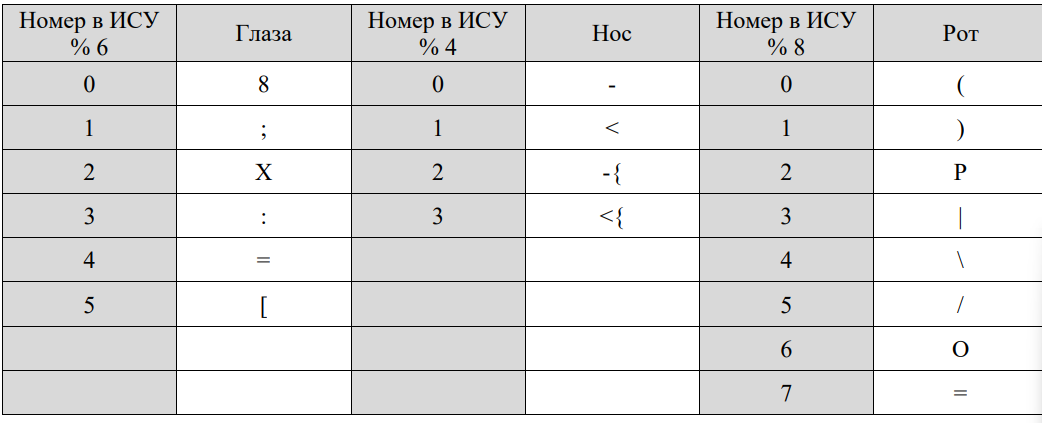
\includegraphics[scale=0.7]{task_1}
\end{figure}

\subsection*{Тестовые файлы}
\subsubsection*{Тест 1}
\textit{Lorem [</ ipsum odor amet, consectetuer [</adipiscing elit.}

\subsubsection*{Тест 2}
\textit{Cra[</s eu auctor mus, ve[</hicula mass[</a ligula.}

\subsubsection*{Тест 3}
\textit{Nulla pellentesque turpis [</ dictum accumsan tortor ac.}

\subsubsection*{Тест 4}
\textit{Sit senectus acc[</umsan ultricies ac nasce[</tur mus quis taciti}

\subsubsection*{Тест 5}
\textit{In curabitur ante dolor; torquent[</ erat [</sagittis [</cras fermentu[</m.}

\subsection*{Вычислятор смайликов}
\begin{minted}[breaklines]{python}
EYES = ("8", ";", "X", ":", "=", "[")
NOSE = ("-", "<", "-{", "<{")
MOUTH = ("(", ")", "P", "|", "\\", "/", "O", "=")
		
		
def get_isu() -> int:
    raw = input("Введите свой ISU: ")
    if not raw.isdigit():
        raise ValueError("ISU должен состьять из цифр")
    if len(raw) != 6:
        raise ValueError("ISU должен состоять из 6 цифр")

    return int(raw)

		
def calculate_emoji(isu: int) -> str:
    emoji = EYES[isu % 6] + NOSE[isu % 4] + MOUTH[isu % 8]

    return emoji
		
		
def main() -> None:
    isu = get_isu()
    emoji = calculate_emoji(isu)
		
    print(f"Ваш смайлик: {emoji}")
		
		
if __name__ == "__main__":
    main()

\end{minted}

\subsection*{Листинг}
\begin{minted}[breaklines]{python}
import re
from pathlib import Path

TEXTS_PATH = Path(__file__).parent / "texts" / "task_1"
EMOJI_PATTERN = re.compile(r"\[</")

CORRECT_COUNTS = (1, 3, 1, 2, 4)


def count_emoji(text: str) -> int:
    return len(EMOJI_PATTERN.findall(text))


def main() -> None:
    for i in range(1, 6):
        text = (TEXTS_PATH / f"text_{i}").read_text()
        emoji_count = count_emoji(text)

        if emoji_count != CORRECT_COUNTS[i - 1]:
            print(
                f"Ошибка в тесте {i}. "
                f"Ожидалось - {CORRECT_COUNTS[i - 1]}, "
                f"найдено - {emoji_count}"
            )
        else:
            print(f"Текст {i}: смайликов - {emoji_count}")
        print("=" * 100)


if __name__ == '__main__':
    main()
\end{minted}

